% Chapter 2

\chapter{Methodology for Data Joins} \label{c2} % Main chapter title

%\label{Chapter1} % For referencing the chapter elsewhere, use \ref{Chapter1} 

%----------------------------------------------------------------------------------------

% Define some commands to keep the formatting separated from the content 
\newcommand{\keyword}[1]{\textbf{#1}}
\newcommand{\tabhead}[1]{\textbf{#1}}
\newcommand{\code}[1]{\texttt{#1}}
\newcommand{\file}[1]{\texttt{\bfseries#1}}
\newcommand{\option}[1]{\texttt{\itshape#1}}

%----------------------------------------------------------------------------------------
\section{Software Structure}\label{s2.ss}

Based on the shortcomings of the different techniques we discussed in the previous sections, we will try to develop a tool that will not only attack the biggest limitation we have found (intuitiveness), but this tool will also be user friendly. This will allow users who have no experience in data joins to create  animations which are easy to understand by just clicking a few buttons, and also provide a support for those who are currently teaching joins.  \\

To create the animations, two programming languages were used, \textsf{R} and \textsf{JavaScript}. \textsf{HTML} and \textsf{CSS} were also used but they are considered to be a markup language and a style sheet language. \textsf{R} was used to process the data, display the animations and provide an interactive dashboard. \textsf{JavaScript} was used to create the animations. Lastly, \textbf{htmlwidgets} \citep{htmlwidgets} is a tool which allows \textsf{R} and \texsf{JavaScript} to communicate with each other and \textbf{shiny} \citep{shiny} is a tool used to create the interactive dashboard.

\begin{figure}[H]
    \centering
    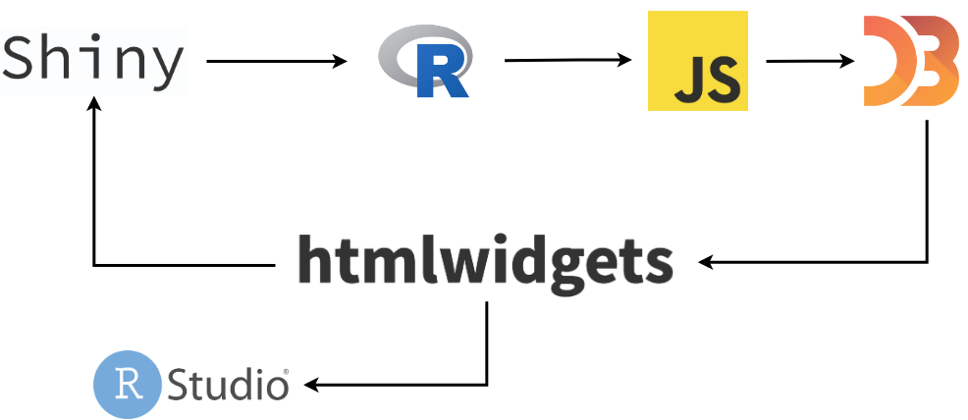
\includegraphics[scale = 0.9]{Masters-Thesis/img/softflow.png}
    \caption{Software Structure}
    \label{fig:softflow}
\end{figure}

We are creating dynamic visualisations that can be delivered over the internet that are made using our \textbf{shiny} app, and that take user instructions and display the resulting dynamic graphics. The graphics are created using \textsf{JavaScript}, and in particular the \textbf{D3} library which provides very useful tools for creating new free-form graphics to display in a browser.  An \textsf{R} function called \texttt{join\_anim} function from our \textbf{dataAnim} package takes the user instructions communicated via the \textbf{shiny} dashboard, reads in the data sets to be joined, pre-processes the data, and then compiles a set of instructions to be fed to our \textsf{JavaScript} program.  The \textsf{JavaScript} program creates the graphics which are then passed back to \textbf{shiny} for display. The graphics can be saved as a (dynamic) \textbf{HTML} file that can be given away and used independently of the system. \\

The first step of the animation is to process the data in \textbf{R} by using \textbf{dplyr} \citep{dplyr}, a package for data manipulation. It provides useful functions to both manipulate and join the data sets. Next this information will be passed to \textsf{JavaScript}, where we use \textbf{D3}, a powerful graphing library for creating animations. After the JavaScript creates the animation in a SVG format, we then use \textbf{htmlwidgets} in \textsf{R} to wrap the SVG up in a container which lets us display them in a browser or the view panel in \textbf{Rstudio}. What \textbf{htmlwidgets} also provides is to render the animation into an object that \textbf{shiny} can take in. This is useful because we are  creating our interactive dashboard in Shiny. \\

With this tool, users will be able to create animations in \textbf{Rstudio} by using the console, or in \textbf{shiny} by using the user interface. On top of that, users will be able to save animations they create, based on their own data sets, in a \textbf{HTML} format. This is useful because they will be able to share these animations with other people.

\section{R}
Mainly, two packages were used in \textsf{R}, \textbf{dplyr} and \textbf{tidyr} \citep{tidyr}. Both packages were used to manipulate and transform data sets provided by the user, so we can extract information shown below to pass into \textsf{JavaScript}. 

What happens is when the user input the data sets, \textsf{R} processes it and produces a list of step by step instructions of how the animations are to be created for \textsf{JavaScript}. Some examples are, column one from Table 1 and column two from Table 2 are the key columns. Row one from Table 1 matches row three from Table 2. \\

Other information passed to JavaScript from R includes: 
\begin{itemize}
    \item The dimensions and information of the two input tables, and the joined table
    \item The size of the tables in the animation
    \item The order and the corresponding matching rows throughout the joining animation
    \item The text of the instructional messages to be displayed when they are required
    \item How to deal with unmatched rows for different kind of joins
\end{itemize}

\newpage 

\section{New package - dataAnim}
To produce the joining animations, the \texttt{join\_anim} function in our \href{https://github.com/chrk623/dataAnim}{\textbf{dataAnim}} package is used. The compulsory arguments are the type of join to perform, the two tables and the key column to join by. 
Optional arguments include the speed of the animation and a logical value to choose whether to display the instructional messages. An example of this function is shown in Fig.~\ref{fig:joinanim}.

\begin{figure}[H]
    \centering
    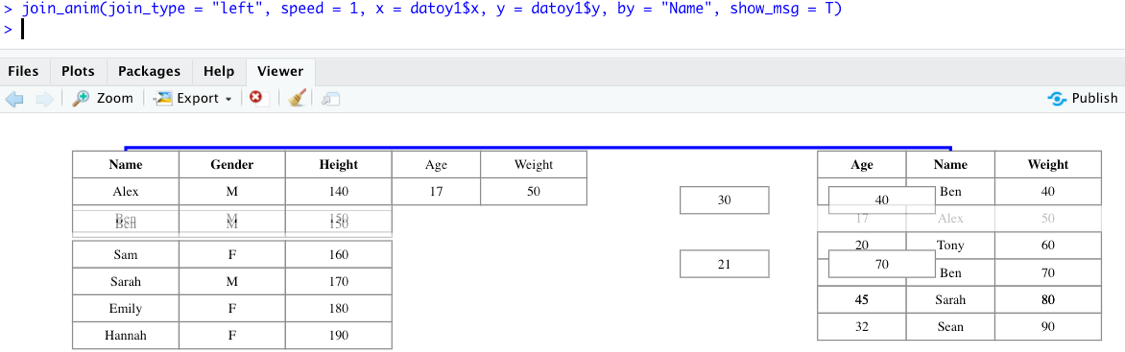
\includegraphics[scale = 0.8]{Masters-Thesis/img/joinanim.png}
    \caption{\texttt{join\_anim} example}
    \label{fig:joinanim}
\end{figure}

Currently, it supports three type of joins, \textit{left join}, \textit{inner join} and \textit{complete join}. A \textit{right join} is basically the same as a \textit{left join}, except that it just joins onto the right table instead of the left table. \textit{Left join} is also known as \textit{left outer join}, and a \text{full join} is also known as a \textit{complete join} or \textit{full outer join}. \\

The \texttt{join\_anim} function returns a \textbf{htmlwidgets} object which the user can use via the \texttt{savewidget} function from \textbf{htmlwidget} to save the object as a \textbf{HTML} file. The help file for The \texttt{join\_anim} function follows in Fig.~\ref{fig:joinanimhelp}. \\

Discussion of the arguments:
\begin{itemize}
    \item \texttt{join\_type} allow users to choose the type of join they want perform.
    \item \texttt{x} and \texttt{y} are the tables that are being joined together.
    \item \texttt{by} is the key column which defines the join.
    \item \texttt{speed} allows us to give the user control of the speed of the animation.
    \item \texttt{width} and \texttt{height} are the size of the animation frame in pixels
    \item \texttt{show\_msg} gives the user an option to include explanatory annotations in the animation.
\end{itemize}

\begin{figure}[H]
    \centering
    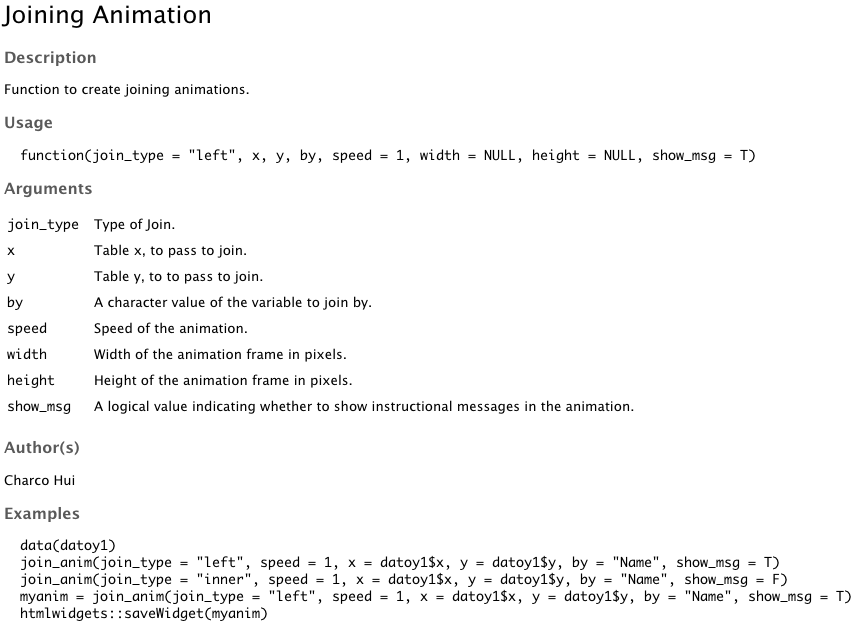
\includegraphics[scale = 0.5]{Masters-Thesis/img/joinanimhelp.png}
    \caption{\texttt{join\_anim} help page}
    \label{fig:joinanimhelp}
\end{figure}



\section{\textsf{JavaScript} - \textbf{D3}}

\textbf{D3} is a popular library in \textsf{JavaScript} to create dynamic interactive data visualisations. \textbf{D3} creates graphics in scalable vector graphics (SVG), a file format based on mathematical calculations. This means that the graphics can be zoomed in without becoming pixelated.  Many famous and influential companies like the New York Times uses this technology to produce interactive or SVG graphics. 

Here, the \textsf{JavaScript} program receives the instructions produced by \textsf{R} and calls \textbf{D3} functions to create the animations, then \textsf{JavaScript} sends the animation in SVG format back to \textsf{R} to process the final presentation. The problem with using \textsf{JavaScript} and \textbf{D3} is that they run asynchronously, meaning that all the code runs at once, this causes problems because there are many components in our animations that are created during the animation. Therefore when the program is created, we need to be cautious and need to make provisions for the new components that are not displayed in the animation originally. A flow of our \textsf{JavaScript} program is shown in Figure~\ref{fig:jsflow}. \\

\begin{figure}[H]
    \centering
    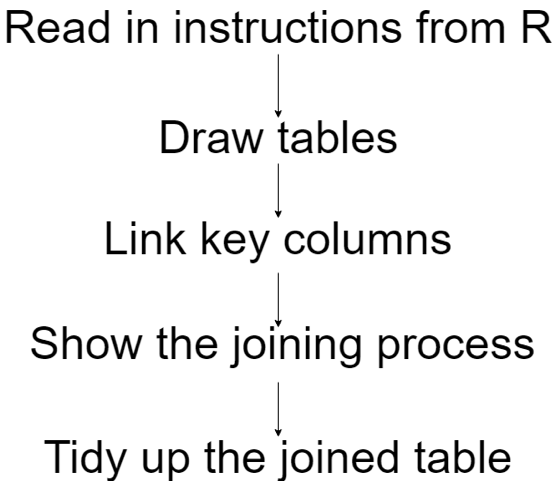
\includegraphics[scale = 1.0]{Masters-Thesis/img/jsflow.png}
    \caption{\textsf{JavaScript} program flow}
    \label{fig:jsflow}
\end{figure}

As shown in the above diagram, the \textsf{JavaScript} program:

\begin{enumerate}
    \item Reads in the instruction from \textsf{R} and passing \textsf{R} objects directly to \textsf{JavaScript} using the \textbf{htmlwidgets} environment.
    \item Draws the two tables, at the correct co-ordinates.
    \item Implements animation to show which columns are the key columns from each table, and links them together.
    \item Starts the joining animation by the type of join the user chose. Instructional messages explaining each steps will also be shown unless the user chooses not to.
    \item Tidy up the joined table. At the end the table that we are joining from will fade out, and the joined table will stay. The joined table will then move to the middle indicating that it is the completed table and that the animation is over.
\end{enumerate}

\section{\textbf{htmlwidgets} and \textbf{shiny}}

As discussed at the start of this chapter, the \textsf{JavaScript} program uses \textbf{D3} to creates graphics and animations in SVG, which are mostly displayed in internet browsers. Natively, \textsf{R} does not support SVG graphics directly, so, to display the animations in \textsf{R}, we need to use \textbf{htmlwidgets}. The \textbf{shiny} interactive dashboard for the users, is shown in Fig.~\ref{fig:shinydash}. This is a good extension because this will allow users who have no experience in programming to create the animations by using the command panel displayed in Fig.~\ref{fig:shinydash}.

\begin{figure}[H]
    % \centering
    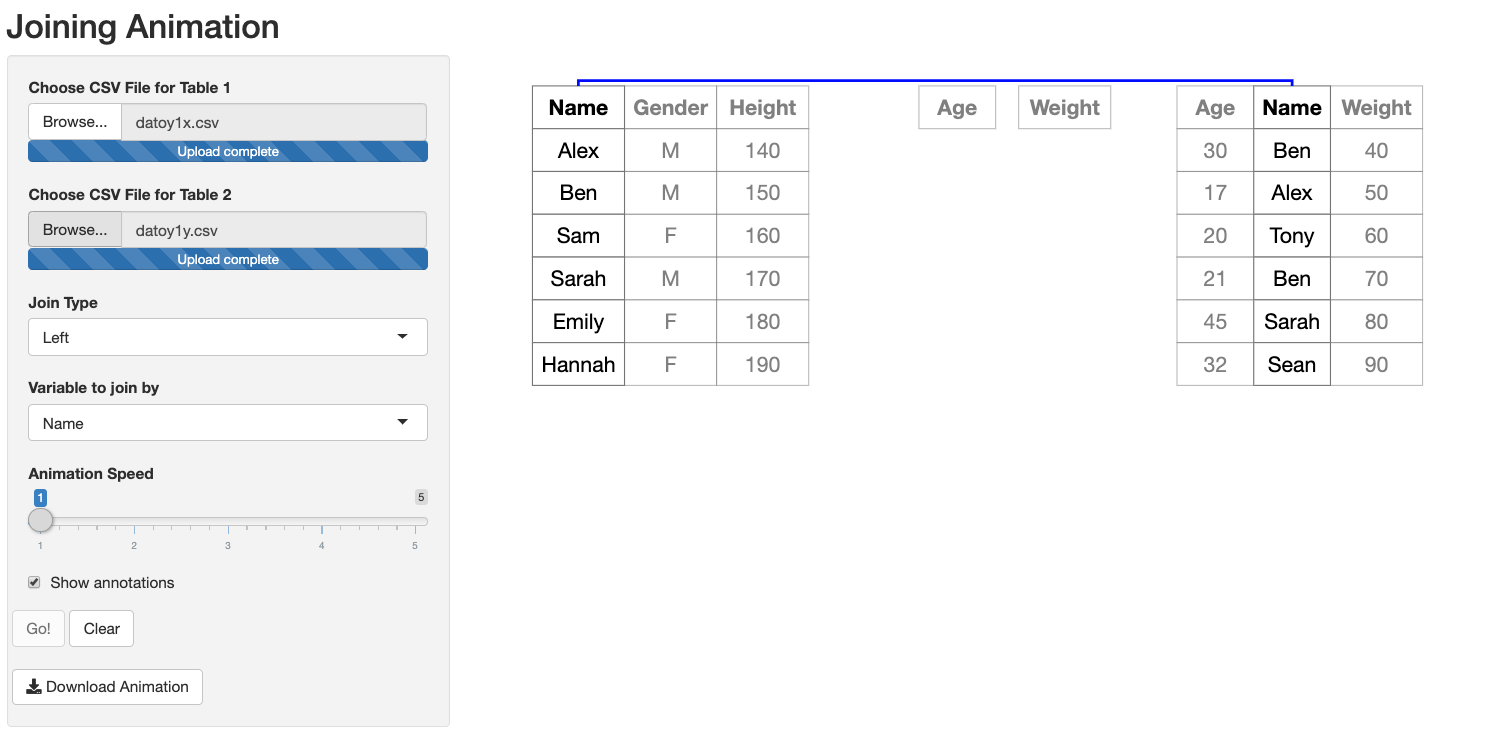
\includegraphics[scale = 0.3]{Masters-Thesis/img/shinydash.png}
    \caption{ \textbf{shiny} interactive dashboard in \textbf{dataAnim}}
    \label{fig:shinydash}
\end{figure}

\section{Animation}

In the previous section, some issues with the existing approach of teaching data joins were discussed. Some improvements were made to address those issues, with the end goal of making these animations as intuitive as possible. 

The goals of these animations are to:

\begin{itemize}
    \item To show the logic of the joins
    \item Highlight the importance and role of the key variables
    \item Show the user how each of the rows are being joined together
    \item Show how the joins handle unmatched rows
    \item Show how the joins handle multiple matches
    \item Show how data are moved between tables
    \item Show how different type of joins handle the tables differently.
    \item Allow users to download and export the animations.
\end{itemize}